\begin{titlepage}
\chapter{Implementación de la aplicación web}
\section{Descripción general}
El objetivo de la aplicación web es que sirva de interfaz para mostrar los datos recopilados de todos los sensores que se encuentren configurados en la red. 
\section{Implementación backend}
El backend de la aplicación web se ha implementado en Python utilizando el framework Flask, SocketIO y Paho para MQTT. Flask permite crear aplicaciones web de forma rápida y sencilla. SocketIO permite que la aplicación web sea capaz de recibir mensajes en tiempo real y comunicarse de forma facil con el cliente. Paho es una librería para MQTT que permite conectarse a un broker MQTT y publicar y suscribirse a topics.
\subsection{Aplicación en python3}
\subsubsection{Configuración de Flask}
Con la siguiente configuración, creamos una aplicación FLask pudiendo indicarle a la vez toda la configuración MQTT a usar.
\begin{lstlisting}[language=python]
	app = Flask(__name__)
	app.config['SECRET'] = 'my secret key'
	app.config['TEMPLATES_AUTO_RELOAD'] = True
	app.config['MQTT_BROKER_URL'] = '192.168.1.200'
	app.config['MQTT_BROKER_PORT'] = 1883
	app.config['MQTT_CLIENT_ID'] = 'APP_SERVER'
	app.config['MQTT_CLEAN_SESSION'] = True
	app.config['MQTT_USERNAME'] = 'pi'
	app.config['MQTT_PASSWORD'] = 'nairda'
	app.config['MQTT_KEEPALIVE'] = 5
	app.config['MQTT_TLS_ENABLED'] = False
	app.config['MQTT_LAST_WILL_TOPIC'] = 'home/lastwill'
	app.config['MQTT_LAST_WILL_MESSAGE'] = 'bye'
	app.config['MQTT_LAST_WILL_QOS'] = 2
\end{lstlisting}

\subsubsection{Background tasks}
Esta clase se encarga de ejecutar las tareas en segundo plano. Una tarea ira actualizando periodicamente el coste de la electricidad, y la otra tarea se ejecutara cuando sea necesario enviar la configuración a un sensor por MQTT.\\
\begin{lstlisting}[language=python]
class backgroundTask():
    def __init__(self):
        self.sendConfigToSensor = False

    def stop_sendConfigToSensor(self):
        logging.debug('stop_sendConfigToSensor called')
        self.sendConfigToSensor = False

    def start_sendConfigToSensor(self, json_data):
        self.sendConfigToSensor = True
        data = json.loads(json_data)
        logging.info("Starting background thread to send config to sensor")
        while self.sendConfigToSensor:
            logging.info("Running loop to send config to sensor")
            logging.info('Sending config to sensor %s', \
			data['sensor_type'] + ',' + data['voltage'])
            mqtt.publish('sensor_config/' + data['sensor_id'], \
			data['sensor_type'] + ',' + data['voltage'])
            socketio.sleep(1)
    
    def update_cost_electricity(self):
        
        while True:
            costElectricity.load_current_data()
            logging.debug("Reloading cost electricity data :", 
			costElectricity.current_data)
            #notify socket new data
            socketio.emit('cost_electricity', costElectricity.current_data)
            socketio.sleep(60)
\end{lstlisting}

\subsubsection{Clase para gestionar los sensores}
Esta clase se encarga de gestionar los sensores, almacenando los datos de los sensores en un JSON. Tenemos una para añadir un sensor al JSON, otra función para leer los sensores del JSON y otra para eliminar un sensor del JSON.\\

\begin{lstlisting}[language=python]
class handleSensors():
    def __init__(self):
        self.JSON_FILE = 'sensors.json'
        self.sensors_data = None
    
    def read_saved_sensors(self):
        if os.path.isfile(self.JSON_FILE):
            with open(self.JSON_FILE, "r") as f:
                self.sensors_data = json.load(f)
                print(self.sensors_data)
        else:
            with open(self.JSON_FILE, "w", encoding='utf-8') as f:
                json.dump({}, f, ensure_ascii=False, indent=4)
            logging.debug("No sensors found")

    def add_sensor(self, sensor):
        with open(self.JSON_FILE, "r") as f:
            json_sensors = json.load(f)
            sensorFound = False
            for sensor_id, sensor_data in json_sensors.items():
                print("sensor_id: ", sensor_id, "sensor_type: ", 
				sensor_data["sensor_type"])

            if not sensorFound:
                logging.debug("New sensor added: %s", sensor["sensor_id"])
                json_sensors[sensor["sensor_id"]] = sensor
                self.sensors_data = json_sensors
                with open(self.JSON_FILE, "w", encoding='utf-8') as f:
                    json.dump(json_sensors, f, ensure_ascii=False, indent=4)
                #after adding, subscribe to watts topic
                mqtt.subscribe('watts/' + sensor["sensor_id"])
    
    def remove_sensor(self, sensor_id):
        with open(self.JSON_FILE, "r") as f:
            json_sensors = json.load(f)
            json_sensors.pop(sensor_id)
            self.sensors_data = json_sensors
            with open(self.JSON_FILE, "w", encoding='utf-8') as f:
                json.dump(json_sensors, f, ensure_ascii=False, indent=4)
            #after removing, unsubscribe to watts topic
            mqtt.unsubscribe('watts/' + sensor_id)
\end{lstlisting}

\subsubsection{Funciones de la APP FLask}
Cada vez que un cliente pida una dirección de la web, estas son las funciones que se ejecutan, que tan solo llaman a renderizar plantillas html.\\
\begin{lstlisting}[language=python]
@app.route('/')
def index():
	return render_template('index.html')

@app.route('/add_sensor')
def add_sensor():
	return render_template('add_sensor.html')

@app.route('/sensors')
def sensors():
	print("sensors " + str(handleSensors.sensors_data))
	return render_template('sensors.html', 
	sensors=handleSensors.sensors_data)

@app.route('/sensors/<path:sensor_id>')
def sensor(sensor_id):
	return render_template('display_sensor_data.html', 
	data=handleSensors.sensors_data[sensor_id])
\end{lstlisting}

\subsubsection{Llamadas a socketio}
Estas son las llamadas a socketio que se ejecutan cuando se produce un evento. Para cada evento, se ejecutan diferentes acciones. Los eventos los pueden haber generado los clientes o la propia aplicación llamando a socketio.emit('EVENTO').\\
\begin{lstlisting}[language=python]
@socketio.on('publish')
def handle_publish(json_str):
	data = json.loads(json_str)
	mqtt.publish(data['topic'], data['message'], data['qos'])


@socketio.on('subscribe')
def handle_subscribe(json_str):
	data = json.loads(json_str)
	mqtt.subscribe(data['topic'], data['qos'])

@socketio.on('submit_sensor')
def handle_submit_sensor(json_str):
	data = json.loads(json_str)
	logging.info("New sensor added: %s", data['sensor_id'])
	mqtt.publish('ack/' + data['sensor_id'], "ack", 0)
	backgroundTask.start_sendConfigToSensor(json_str)
	handleSensors.add_sensor(data)

@socketio.on('stop_sending_config')
def handle_stop_sending_config():
	backgroundTask.stop_sendConfigToSensor()

@socketio.on('reset_sensor')
def handle_reset_sensor(str):
	logging.debug("Reset sensor: %s", str)
	mqtt.publish('restart/' + str, "restart", 0)

@socketio.on('calibrate_sensor')
def handle_calibrate_sensor(str):
	logging.debug("Recalibrating sensor: %s", str)
	mqtt.publish('calibrate/' + str, "reset", 0)

@socketio.on('delete_sensor')
def handle_delete_sensor(str):
	logging.debug("Deleting sensor: %s", str)
	handleSensors.remove_sensor(str)
	mqtt.publish('reset/' + str, "reset", 0)

@socketio.on('unsubscribe_all')
def handle_unsubscribe_all():
	mqtt.unsubscribe_all()

@socketio.on('unsubscribe_sensor_id')
def handle_unsubscribe_sensor_id():
	mqtt.unsubscribe('clientID/broker')

@socketio.on('connect')
def handle_connect():
	logging.info("Client connected")
	socketio.start_background_task(backgroundTask.update_cost_electricity)

\end{lstlisting}

\subsubsection{Funciones de MQTT}
Cada vez que recibamos un mensaje en uno de los topics a los que se haya suscrito la app, se ejecutara la función on\_message. Para cuando MQTT se conecta al broker, se ejecuta la función on\_connect que lo unico que hace es suscribirse al topic de cada sensor para recibir los datos de consumo.\\
\begin{lstlisting}[language=python]
@mqtt.on_message()
def handle_mqtt_message(client, userdata, message):
	data = dict(
		topic=message.topic,
		payload=message.payload.decode(),
		qos=message.qos,
	)
	print("message received: ", data)
	socketio.emit('mqtt_message', data=data)

@mqtt.on_connect()
def handle_mqtt_connect(client, userdata, flags, rc):
	for sensor, data in handleSensors.sensors_data.items():
		logging.debug("Subscribing to sensor: %s", sensor)
		mqtt.subscribe('watts/' + sensor, 0)
\end{lstlisting}

\subsubsection{Clase para obtener precio KWh}
Para obtener el precio del KWh se ha utilizado la API de la web de https://api.preciodelaluz.org/. Esta API devuelve el precio del KWh en tiempo real.
\begin{lstlisting}[language=python]
import requests
import json


class costElectricity:
    """
    Class to get the price of electricity in Spain
    """
    def __init__(self):
        self.url_complete   = 
		'https://api.preciodelaluz.org/v1/prices/all?zone=PCB'
        self.url_average    = 
		'https://api.preciodelaluz.org/v1/prices/avg?zone=PCB'
        self.url_max        = 
		'https://api.preciodelaluz.org/v1/prices/max?zone=PCB'
        self.url_min        = 
		'https://api.preciodelaluz.org/v1/prices/min?zone=PCB'
        self.url_current    = 
		'https://api.preciodelaluz.org/v1/prices/now?zone=PCB'
        self.url_eco        = 
		'https://api.preciodelaluz.org/v1/prices/cheapests?zone=PCB&n='
        self.complete_data  = None
        self.average_data   = None
        self.max_data       = None
        self.min_data       = None
        self.current_data   = None

    
    def get_url_data(self, url):
        response = requests.get(url)
        if response.status_code == 200:
            return json.loads(response.text)
        else:
            print("Error  getting data from " + url)
            return None


    def load_complete_data(self):
        self.complete_data = self.get_url_data(self.url_complete)

    def load_average_data(self):
        self.average_data = self.get_url_data(self.url_average)
    
    def load_max_data(self):
        self.max_data = self.get_url_data(self.url_max)
    
    def load_min_data(self):
        self.min_data = self.get_url_data(self.url_min)
    
    def load_current_data(self):
        self.current_data = self.get_url_data(self.url_current)

    def update_everything(self):
        self.load_complete_data()
        self.load_average_data()
        self.load_max_data()
        self.load_min_data()
        self.load_current_data()

    """ Returns a list of the n cheapest prices in the day """
    def get_eco_price(self, n):
        return self.get_url_data(self.url_eco + str(n))

\end{lstlisting}

\subsubsection{Inicialización de la aplicación}
\begin{lstlisting}[language=python]
if __name__ == '__main__':
	handleSensors.read_saved_sensors()
	costElectricity.load_current_data()
	socketio.run(app, host='localhost', port=5000, use_reloader=False, debug=True)
\end{lstlisting}

El codigo completo se puede consultar en el repositorio de GitHub\cite{ref25}
\section{Implementación frontend}
\subsection{Diseño}
\subsubsection{Añadir sensor}
Cosas a destacar de la interfaz de añadir un sensor:
\begin{itemize}
	\item El boton de busqueda hará que si hay algun sensor publicando su ID en el topic correspondiente, se añadirá automaticamente al campor "Sensor ID".
	\item Podemos elegir el tipo de sensor que estamos añadiendo, es decir, podremos elegir entre el sensor ACS712 de 5A, el de 20A o el de 30A.
	\item Otra cosa que debemos configurar bien es el "Load voltage", es decir, la tensión a la que se le aplica la carga al sensor. Esto es importante ya que el sensor ACS712 necesita saber la tensión a la que se le aplica la carga para poder calcular el consumo electrico correctamente.
	\item Una vez le demos al boton de Añadir, el servidor enviará la configuración al esp32 que corresponda.
\end{itemize}
\begin{figure}[h!]
	\centering
	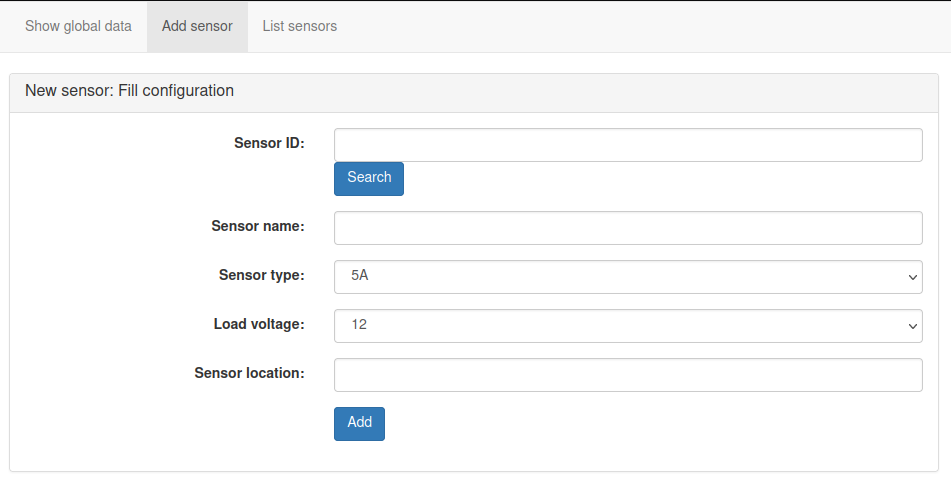
\includegraphics[width=1\textwidth]{imagenes/web_addsensor.png}
	\caption{Interfaz para añadir un sensor}
\end{figure}
\subsubsection{Mostrar sensores}
Aquí simplemente saldrá una lista de los sensores que haya configurados.
\begin{figure}[h!]
	\centering
	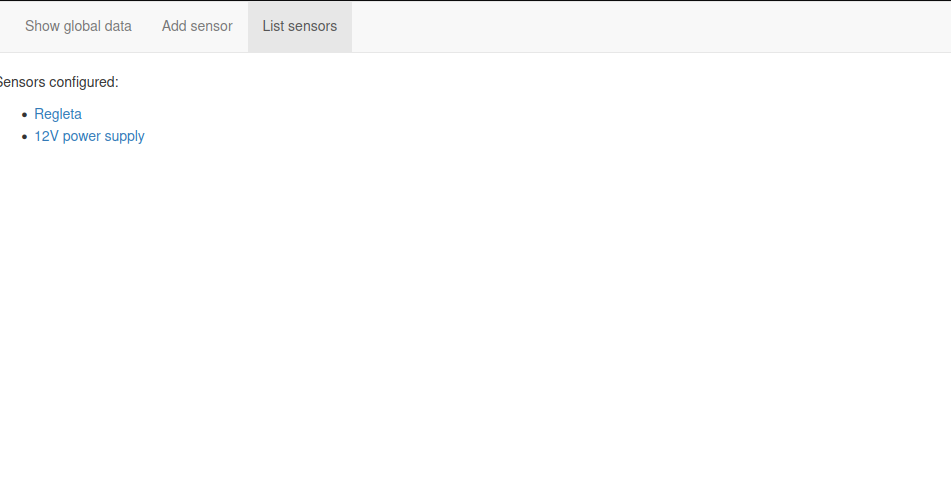
\includegraphics[width=1\textwidth]{imagenes/web_listsensors.png}
	\caption{Interfaz para mostrar los sensores añadidos}
\end{figure}
\subsubsection{Mostrar datos de un sensor}
En esta interfaz se mostrarán los datos del sensor elegido. Por un lado tenemos una grafica que va mostrando en tiempo real los datos que se van recibiendo del sensor en Watts. Por otro lado podemos ver una tabla con los datos del consumo actual, el coste en euros del consumo actual, el precio del KWh y el consumo total en KWh. Tambien tenemos un cuadro con la información del sensor y unos botones para enviar un reset al esp32, que se calibre de nuevo el sensor y para eliminar el sensor configurado. Por ultimo se muestra una especie de consola con los ultimos 20 valores recibidos del sensor. 
\begin{figure}[h!]
	\centering
	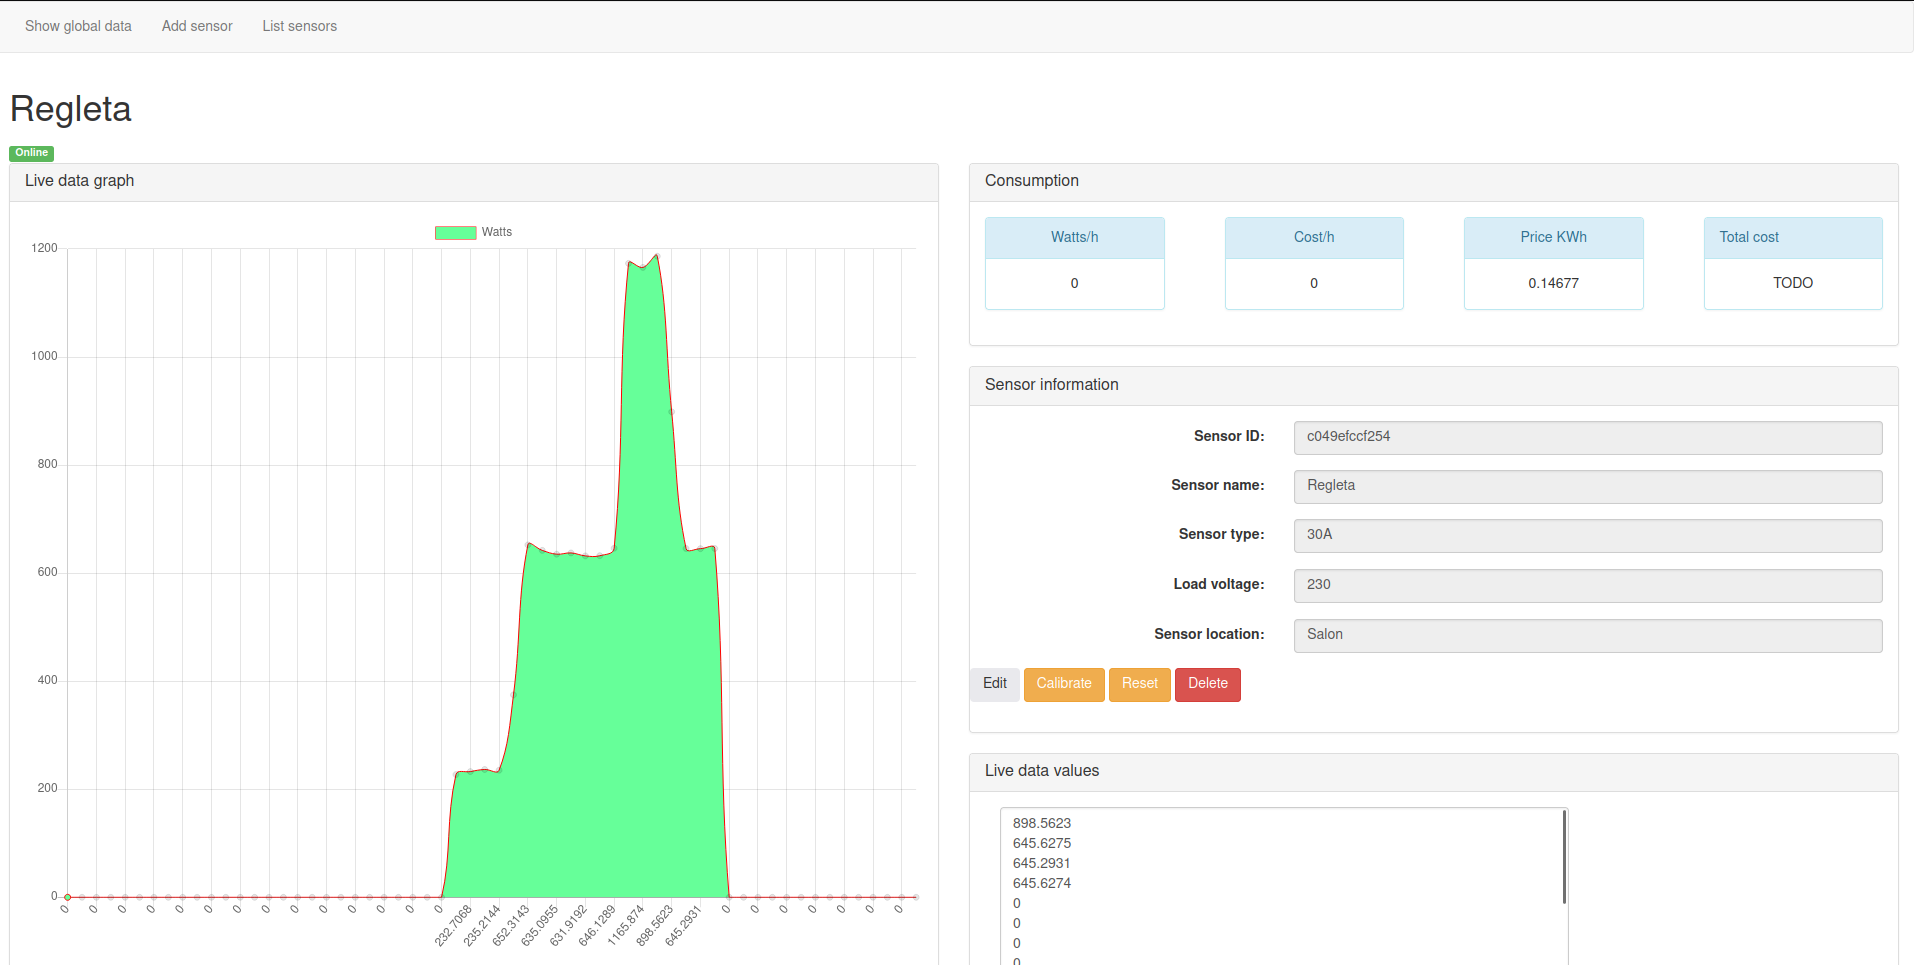
\includegraphics[width=1\textwidth]{imagenes/web_datos.png}
	\caption{Interfaz para mostrar los datos de un sensor}
\end{figure}
\subsection{Implementación}
Para la implementación del frontend se ha usado html, javascript y bootstrap. El codigo completo se puede consultar en el repositorio de GitHub\cite{ref25} en la carpeta de templates.


\end{titlepage}
